\documentclass[tikz,border=8pt]{standalone}
\usepackage[scaled=0.95]{helvet}
\renewcommand{\familydefault}{\sfdefault}
\usetikzlibrary{arrows.meta}
\definecolor{TEJNavy}{HTML}{1E2B55}
\definecolor{TEJBlue}{HTML}{1769AA}
\definecolor{TEJRed}{HTML}{B3261E}
\begin{document}
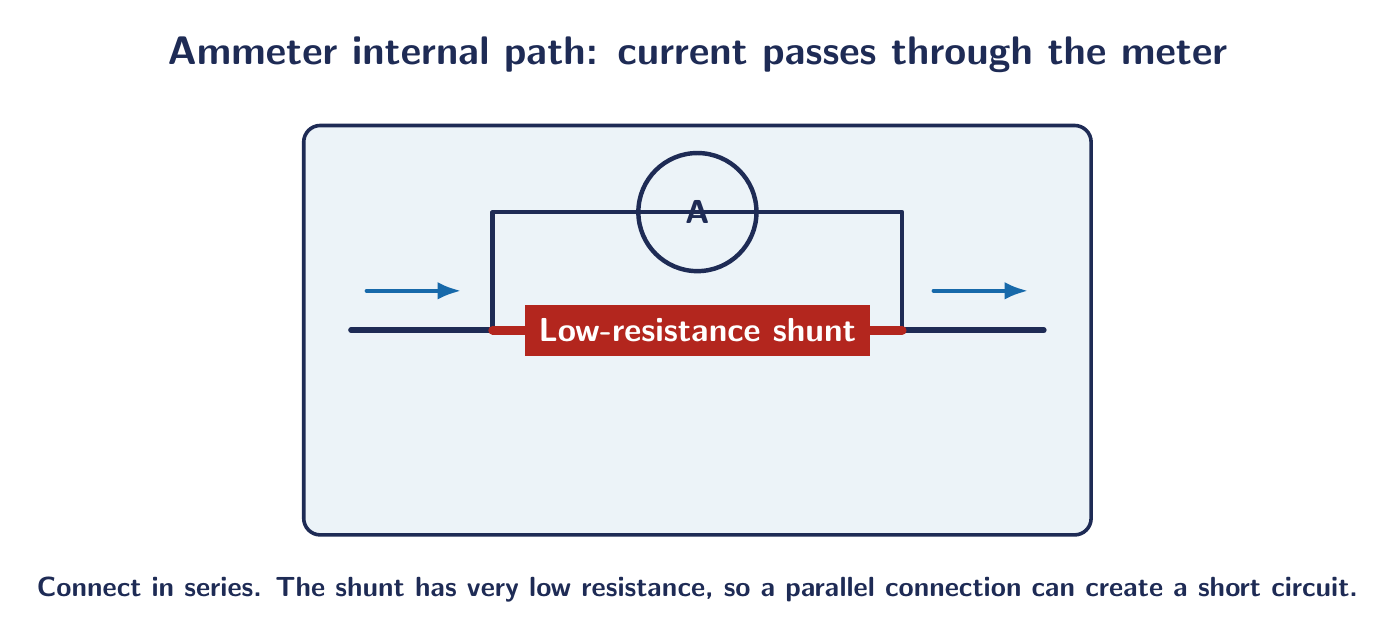
\begin{tikzpicture}[line cap=round,line join=round,font=\sffamily]
  \filldraw[fill=TEJBlue!8,draw=TEJNavy,line width=1.3pt,rounded corners=6pt] (0,0) rectangle (10,5.2);
  \draw[TEJNavy,line width=2pt] (0.6,2.6) -- (2.4,2.6);
  \draw[TEJNavy,line width=2pt] (7.6,2.6) -- (9.4,2.6);
  \draw[TEJNavy,line width=1.6pt] (2.4,2.6) -- (2.4,4.1) -- (7.6,4.1) -- (7.6,2.6);
  \draw[TEJRed,line width=3.2pt] (2.4,2.6) -- (7.6,2.6);
  \draw[TEJNavy,line width=1.6pt] (5,4.1) circle (0.75);
  \node[font=\bfseries\Large,text=TEJNavy] at (5,6.1) {Ammeter internal path: current passes through the meter};
  \node[font=\bfseries\large,text=white,fill=TEJRed,inner sep=5pt] at (5,2.6) {Low-resistance shunt};
  \node[font=\bfseries\large,text=TEJNavy] at (5,4.1) {A};
  \draw[-{Latex[length=3mm]},TEJBlue,line width=1.5pt] (0.8,3.1) -- (2.0,3.1);
  \draw[-{Latex[length=3mm]},TEJBlue,line width=1.5pt] (8.0,3.1) -- (9.2,3.1);
  \node[font=\bfseries,text=TEJNavy,align=center] at (5,-0.7) {Connect in series. The shunt has very low resistance, so a parallel connection can create a short circuit.};
\end{tikzpicture}
\end{document}
